\documentclass{bmvc2k}
\usepackage{amsmath,amssymb}

%% Enter your paper number here for the review copyu
\bmvcreviewcopy{422}

% define title here so headers are updated, too
\def\ttl{Estimating Orientation of Curvilinear Structure}

\title{\ttl}

% Enter the paper's authors in order
% \addauthor{Name}{email/homepage}{INSTITUTION_CODE}
\addauthor{Susan Student}{http://www.vision.inst.ac.uk/~ss}{1}
\addauthor{Petra Prof}{http://www.vision.inst.ac.uk/~pp}{1}
\addauthor{Colin Collaborator}{colin@collaborators.com}{2}

% Enter the institutions
% \addinstitution{Name\\Address}
\addinstitution{
 The Vision Institute\\
 University of Borsetshire\\
 Wimbleham, UK
}
\addinstitution{
 Collaborators, Inc.\\
 123 Park Avenue,\\
 New York, USA
}

\runninghead{Student, Prof, Collaborator}{\ttl}

% Any macro definitions you would like to include
% These are not defined in the style file, because they don't begin
% with \bmva, so they might conflict with the user's own macros.
% The \bmvaOneDot macro adds a full stop unless there is one in the
% text already.
\def\eg{\emph{e.g}\bmvaOneDot}
\def\ie{\emph{i.e}\bmvaOneDot}
\def\Eg{\emph{E.g}\bmvaOneDot}
\def\etal{\emph{et al}\bmvaOneDot}

% macros for referencing figures, tables, equations and sections
\newcommand{\fref}[1]{Figure~\ref{#1}}
\newcommand{\eref}[1]{(\ref{#1})}
\newcommand{\tref}[1]{Table~\ref{#1}}
\newcommand{\sref}[1]{Section~\ref{#1}}
\newcommand{\aref}[1]{Algorithm~\ref{#1}}

% maths macros
\def\G{G}
\def\Gx{G_x}
\def\Gy{G_y}
\def\Gxx{G_{xx}}
\def\Gxy{G_{xy}} \def\Gyx{G_{yx}}
\def\Gyy{G_{yy}}
\def\Ix{I_x}
\def\Iy{I_y}
\def\Ixsqr{I_{x^2}}
\def\Iysqr{I_{y^2}}
\def\Ixx{I_{xx}}
\def\Ixy{I_{xy}}
\def\Iyy{I_{yy}}
\def\dtcwt{DT-$\mathbb{C}$WT}

% command for adding inline comment to text
\newcommand{\comment}[1]{}

%-------------------------------------------------------------------------
% Document starts here
\begin{document}

\maketitle

\begin{abstract}
Estimating orientation of image structure underpins applications including digital mammography, retinography, fingerprint analysis and many more. We consider different choices of filter bank including those based on first and second derivatives, efficient Haar-like features and the Dual Tree Complex Wavelet Transform. We then investigate how standard regressors (linear regression, Boosting and Random Forests) may be adapted to use the responses to these filter banks in order to predict orientation of image structure. For a quantitative evaluation, we use synthetic images based on mammograms and the publicly available DRIVE database of retinal images, and show that Random Forests and the wavelet transform offer superior accuracy though at a cost in efficiency. Qualitative results are also presented for real mammograms and fingerprint images.
\end{abstract}

%-------------------------------------------------------------------------

\def\figpath{./figs}

\section{Introduction}
\label{s:introduction}
Curvilinear structures are important in many applications of computer vision, including aerial image analysis (roads, rivers, railways), fingerprint analysis (ridges) and medical image analysis (blood vessels, ducts). As a result, there is an extensive literature on detecting such structure~\cite{Papari_Petkov_IVC11}. The literature on estimating the local orientation of curvilinear structure is more limited though the problem is equally important, for example as a basis for non-maximal suppression (centre-line detection) and for characterising properties such as tortuosity (\eg~of blood vessels).

In mammography, malignant lesions often exhibit linear structures (known as spicules) that form a radial pattern around the central mass. Detecting linear structures and determining their orientation~\cite{Zwiggelaar_etal_MIA99,Zwiggelaar_etal_TMI04} can therefore indicate points where they converge and thus whether a mass or architectural distortion is present~\cite{Karssemeijer_teBrake_TMI96,Rangayyan_Ayres_MBEC06}. In other medical applications such as retinography (\fref{f:retinography}), the rate of change of orientation (\ie~tortuosity) of blood vessels can serve as a diagnostic indicator of vascular disease~\cite{Hart_etal_IJMI99}; though studies have shown that vessels can be detected and segmented~\cite{Staal_etal_TMI04,Ricci_Perfetti_TMI07,Dabbah_etal_MICCAI10}, few have addressed the problem of measuring their orientation and quantifying tortuosity.

Similarly, automatic fingerprint analysis typically begins by computing the orientation at each pixel via gradient-based filtering, often followed by some smoothing over a local patch~\cite{Bazen_Gerez_TPAMI02,Mei_etal_IVC09}. This orientation field is often parameterized -- via `phase portraits'~\cite{Li_etal_PR06} or polynomial approximation~\cite{Gu_etal_PR04}, for example -- to capture and interpret the underlying properties of the fingerprint such as its `singular points' where the orientation is no longer defined (\eg~at a delta or the centre of a whorl). Though smoothing orientation estimates at a local patch have been the subject of several investigations~\cite{Kass_Witkin_CVGIP87,Rao_Jain_TPAMI92,Perona_TIP98}, we deal only with the initial step of estimating orientation at every pixel.

In this paper we revisit the problem of orientation estimation, reviewing the basic theory, extending the state-of-the-art, and providing the results of extensive evaluation using both real and realistic synthetic images. The first step in estimating orientation usually involves applying a set of linear filters to the image, generally at multiple scales and orientations. As we will show later, the choice of filter-bank has a significant influence on both computational efficiency, and estimation accuracy. Our contribution is to explore the similarities and differences between different approaches, and provide empirical evidence of which work best in practice.

Given a set of filter-bank outputs, the second step in estimating orientation is to combine them in some way. There are two basic approaches: to find the scale at which the total magnitude of response is greatest, and combine the different filter responses at that scale analytically~\cite{Karssemeijer_teBrake_TMI96,Mei_etal_IVC09}; or to use a regression learning approach to combine the filter responses across all scales and orientations~\cite{Berks_etal_IPMI11}. Our contribution is to explore the technical details of orientation regression and provide a comprehensive evaluation of different combinations of filter-bank and analytic/regression methods. Overall we show that an approach based on combining dual-tree complex wavelet filtering with random forest regression achieves significantly better results than any of the other state-of-the-art approaches tested.

\begin{figure}[t]
\centering
\begin{tabular}{c c c}
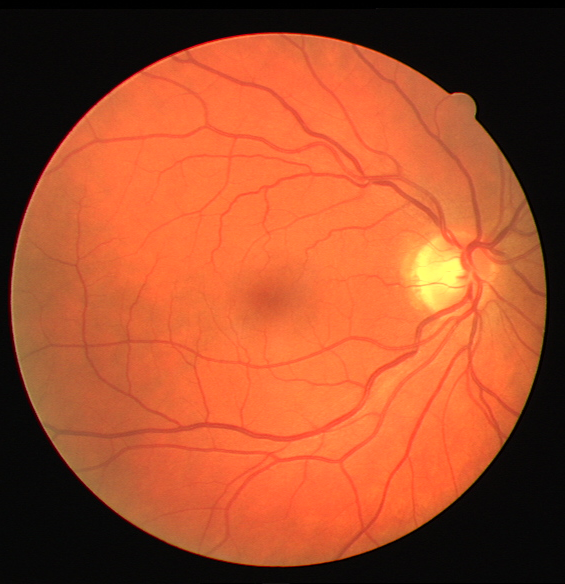
\includegraphics[width=0.3\columnwidth]{\figpath/retina/02_test} &
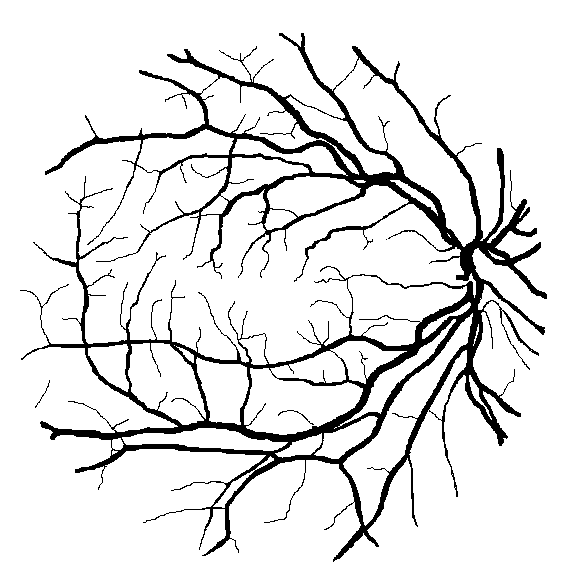
\includegraphics[width=0.3\columnwidth]{\figpath/retina/02_manual1} &
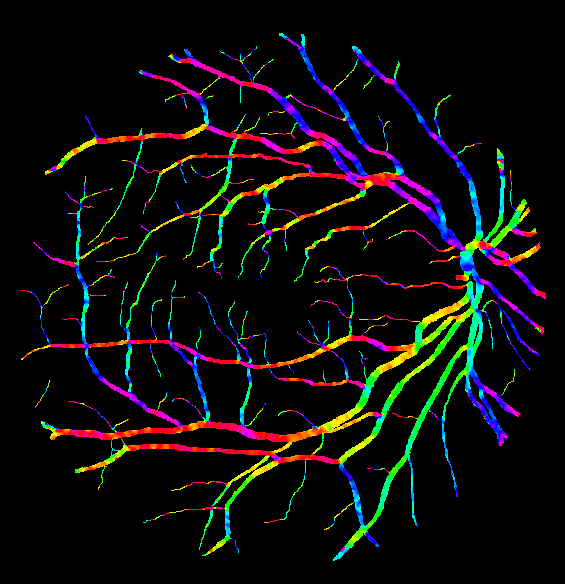
\includegraphics[width=0.3\columnwidth]{\figpath/retina/002_orientation_masked} \\
%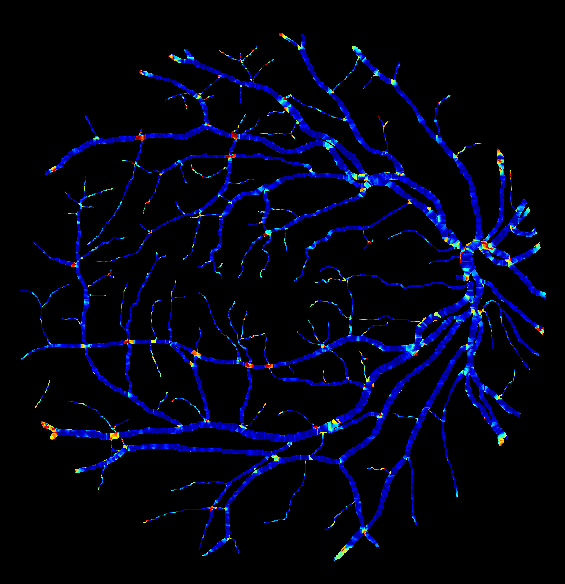
\includegraphics[height=0.15\textheight]{\figpath/retina/002_abs_error} \\
(a) & (b) & (c) \\
\end{tabular}
%
\caption{Estimating orientation in retinography: %
(a) input image; %
(b) ground truth mask indicating pixels belonging to a vessel; %
(c) orientation (indicated by colour) estimated using linear regression over \dtcwt~features. The mask was not used to estimate orientation. %
%(c) magnitude of error (note the regions of high error at points of bifurcation.)
}
\label{f:retinography}
\end{figure}


\section{Image Filtering}
\label{s:filtering}
A simple but na\"ive filtering approach uses smoothed derivatives, $\Gx$ and $\Gy$ (\fref{f:filters}a-b), and their corresponding responses, $\Ix$ and $\Iy$, to compute the direction,

\begin{equation}
\tan^{-1}(\Iy/\Ix),
\label{e:1d}
\end{equation}

\noindent in which gradient is strongest; the perpendicular to this gradient defines the line orientation.

%\begin{figure}
%\centering
%\framebox[0.8\columnwidth][l]{\rule[0.2\textheight]{0pt}{0pt}}
%\caption{Overview image}
%\end{figure}

One problem with this approach is that although the gradient has a clear direction its perpendicular does not (there are two opposite directions, both with zero gradient) and the estimated orientation is arbitrary up to a rotation of $180^\circ$. Though technically we do not distinguish between opposite orientations, opposites cancel when computing statistics (\eg~the mean orientation over a local patch). This can be avoided by multiplying filter responses and instead solving

\begin{equation}
\tan(2\theta) = \frac{2\Ix\Iy}{\Ix^2-\Iy^2}
\label{e:1dsqr}
\end{equation}

\noindent where, by doubling the angle, opposite orientations reinforce each other rather than cancel out~\cite{Mardia_Jupp_00}. A further criticism is that $\Gx$ and $\Gy$ respond most strongly at the edges (rather than the centre) of a bar. In fact, any approach based on odd image filters (\eg~the monogenic signal~\cite{Felsberg_Sommer_TSP01}) fails at the centre of symmetric bar features where both $\Ix$ and $\Iy$ are close to zero such that line orientation is poorly defined.

Taking products of the responses does not help in this respect (the products are also close to zero) but filters based on second derivatives (and that are therefore even) can provide a more stable solution. As noted some years ago (and exploited in mammography applications~\cite{Karssemeijer_teBrake_TMI96}), second derivatives are `steerable' -- the response to a filter at an arbitrary angle can be determined from the responses to three filters at fixed orientations~\cite{Freeman_Adelson_TPAMI91,Koenderink_vanDoorn_TPAMI92} -- and are therefore highly efficient. For further efficiency, we may compute equivalent \emph{separable} filters $\Gxx$, $\Gyy$ and $\Gxy$ (\fref{f:filters}c-e) by differentiating $\Gx$ and $\Gy$, and then determine line orientation by solving

\begin{equation}
\tan(2\theta) = \frac{2\Ixy}{\Ixx-\Iyy}
\label{e:2d}
\end{equation}

\noindent where $\Ixx$, $\Iyy$ and $\Ixy$ are the responses to $\Gxx$, $\Gyy$ and $\Gxy$, respectively. Since \eref{e:1dsqr} and \eref{e:2d} actually give values of $2\theta \pm k\pi$, solving for $\theta$ gives two orientations (one minimum and one maximum) that are $90^\circ$ apart. An analytic solution then requires us to compute the actual response at the two solutions in order to determine which is the direction we want. 

At this point it is helpful to examine the equivalent filters involved: $\Ixy$ and $\Ixx-\Iyy$ (\fref{f:filters}e,f). In particular, we note that their distinctive `cloverleaf' appearance is well approximated by highly efficient Haar-like features (\fref{f:filters}g,h) that have demonstrated success since their introduction for face detection~\cite{Viola_Jones_IJCV04}. To approximate $\Gxx-\Gyy$, we use a modification of the summed area table to compute features at $45^\circ$~\cite{Lienhart_Maydt_ICIP02}.

\begin{figure}[t]
\centering
\begin{tabular}{c c c c}
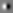
\includegraphics[width=0.15\columnwidth]{\figpath/Gx} &
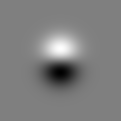
\includegraphics[width=0.15\columnwidth]{\figpath/Gy} &

\includegraphics[width=0.15\columnwidth]{\figpath/Gxx} &
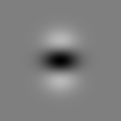
\includegraphics[width=0.15\columnwidth]{\figpath/Gyy} \\
(a) & (b) & (c) & (d) \\
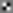
\includegraphics[width=0.15\columnwidth]{\figpath/Gxy} &

\includegraphics[width=0.15\columnwidth]{\figpath/Gxx-Gyy} &

\includegraphics[width=0.15\columnwidth]{\figpath/haar_sin} &

\includegraphics[width=0.15\columnwidth]{\figpath/haar_cos} \\
(e) & (f) & (g) & (h) \\
\end{tabular}
%
\caption{(a,b)~First derivatives, $\Gx$ and $\Gy$; (c-e)~Second derivatives, $\Gxx$, $\Gyy$ and $\Gxy$; (f)~$\Gxx-\Gyy$; (g,h)~Haar-like approximations to $\Gxy$ and $\Gxx-\Gyy$.}
\label{f:filters}
\end{figure}

Although filters based on second derivatives can give accurate output when positioned at the centre of a line feature, accuracy when away from the centre of the line cannot be assured. It has been noted, therefore, that accommodating variation in \emph{phase} of the filter can offer benefits in this regard. Though Gabor filters have historically been a popular choice~\cite{Daugman_TASSP88}, we use a more recent contender known as the Dual-Tree Complex Wavelet Transform (\dtcwt~\cite{Kingsbury_PTRSLA99}). The \dtcwt~has advantages over similar methods in that it combines the computational efficiency of decimation (\ie~multiresolution filtering is achieved by successively down-sampling the image by factors rather than by increasing filter size) whilst still producing approximately shift-invariant coefficients. \dtcwt~coefficients at six directional sub-bands -- oriented at approximately $\pm15^\circ$, $\pm45^\circ$ and $\pm75^\circ$ within each scale -- can be interpolated to obtain a representation of local energy and phase and any spatial location. To achieve $180^\circ$ rotational symmetry, we replace any coefficient with negative imaginary part with its complex conjugate (equivalent to taking the absolute value of the local phase) and adjust the six sub-bands such that the phase at the centre of the impulse response of each wavelet is zero~\cite{Kingsbury_ECSP06,Berks_etal_IPMI11}.

\comment{When dealing with a complex response, $c$, we separate its magnitude, $|c|$, from its phase, $\angle c$. Since orientation is only defined up to a rotation of $180^\circ$, however, a point with phase $\phi$ displaced by $d$ from the centre of a line is indistinguishable from a point with phase $-\phi$ displaced by $-d$ from the same line when looking in the opposite direction; we therefore take the absolute value of phase, $|\angle c|$, at each pixel.}


\subsection{Multiresolution Filtering}
Since curvilinear structure appears at a number of scales in the image (\eg~from fine spicules to thick ducts in mammograms), it is also important to filter the image at several scales to capture all structure~\cite{Lindeberg_IJCV98b}. Having applied our filter bank at a number of scales, an important question is how to interpret the responses at each scale. One option is to discard all scales but that with the strongest overall response~\cite{Karssemeijer_teBrake_TMI96} and use the responses from the discrete orientations at the selected scale to determine orientation analytically. In this work, however, we investigate the alternative approach whereby we use the responses at all scales as input to a regressor that predicts the orientation directly. This general purpose approach has the added advantage that it can be applied for filter banks where an analytic solution is not obvious (such as the \dtcwt).


\section{Estimating Orientation via Machine Learning}
\label{s:learning}
If we have examples of labelled image data for which we wish to estimate orientation, a sensible approach is to compute filter responses (\ie~that form a feature vector) at sampled points in these images and train a regressor to predict the corresponding orientation. We can then apply the trained regressor to a previously unseen image in order to estimate orientation in new cases. Not only is this approach beneficial where an analytic solution is not obvious (as in the \dtcwt) but can also account for factors such as the expected distribution of line widths in a typical image and non-Gaussian noise in medical imaging applications. For the three regressors we use, the targets that we predict are a unit vector in the complex plane where the angle has been doubled (\ie~$t_k = \cos 2\theta_k + i\sin 2\theta_k$) to avoid ambiguity over direction~\cite{Mardia_Jupp_00}. Furthermore, for each pixel we define the feature vector as the responses to all filters pooled over the surrounding $3{\times}3$ pixel region.


\subsection{Linear Regression}
\label{s:learning_linear}
The simplest approach uses a linear regressor such that the predicted output is a weighed sum of the filter responses. Because the outputs are complex the regression coefficients are complex also, though this problem is equivalent to regressing over $\cos 2\theta$ and $\sin 2\theta$ independently.
%Under ideal conditions, applying this method to the real filters (\eg~first and second derivatives) should produce regression coefficients identical to those computed analytically.\comment{Not sure if that is entirely relevant}

%Since the linear regressor minimizes the mean squared error (in $\cos 2\theta$ and $\sin 2\theta$), the uncertainty in the prediction can be represented as an axis aligned Gaussian distribution in the complex plane. If the errors are equally distributed for both $\cos 2\theta$ and $\sin 2\theta$ -- and our experience suggests that they are typically close -- then the angular error (\ie~the angle subtended by isocontours of the Gaussian) is constant for an input of given magnitude; uncertainty is proportionally lower for inputs with larger magnitude, and vice versa. Since phase is limited to the range $[-\pi,\pi)$, however, the magnitude of the feature vector is strongly correlated with the magnitude (rather than phase) of the response to the \dtcwt. As a result, image features with high contrast that respond strongly to the \dtcwt~have lower relative uncertainty (an intuitive result).\comment{This could be considered as 'discussion' and may not be relevant right here}


%\subsection{Logistic Regression}
%\label{s:learning_logistic}
%Since we are predicting sin2T and cos2T, it makes sense to apply some limits to the values these can take. One possibility is to us logistic regression (usually used for classification) which can model a linear region for appropriately scaled targets or a sigmoidal output if necessary. We scale sin and cos to the range [0,1] to learn the regressor and apply the reverse transform on the predictions. This does not restrict outputs to be on (or within) the unit circle but within the unit square.
%
%This is slower to train since it requires iteratively reweighted least squares to minimize the objective function though adds little to testing times.
%Uncertainty will be tricky here


\subsection{Boosted Regression}
\label{s:learning_boosted}
Though straightforward, linear regression breaks down if the relationship between inputs and outputs is in fact nonlinear. Furthermore, the output of a linear regressor is unbounded even though in reality $-1 \leq \sin\theta,\cos\theta \leq 1$. We therefore investigate additive (or \emph{boosted}) regression models that can not only limit output but also capture any nonlinearities in the relationship between feature vector and orientation.

In this work we use an additive model composed of $N=100$ piecewise constant functions. To train the model, we start with a zero residual and iterate the following steps $N$ times: fit a weak predictor to each dimension of the training data in turn; select the dimension and corresponding predictor that minimize the residual error; add a fraction (we use $0.05$) of the prediction to the estimated outputs -- a process known as \emph{shrinkage}~\cite{Friedman_AoS01}; and recompute the residual error. This boosting process is thought to be more insensitive to overtraining than most Machine Learning methods.


\subsection{Random Forest Regression}
\label{s:learning_forest}
Random forests have been shown to be capable of learning complex nonlinear relationships over large numbers of variables (with absolute scales that are incommensurate) at a reasonable computational cost~\cite{Breiman_ML01}. Furthermore, they require little or no tuning and are often resistant to overtraining, making them ideally suited to our regression task. We must be cautious, however, when using trees to predict orientation where vectors close to each other in the complex plane (\eg~$-1+\epsilon i$ and $-1-\epsilon i$) may be confused as being far apart based on their angle alone.

Moreover, splitting dimensions and thresholds are usually chosen based on the variance of the sample either side of the threshold under the assumption of a input Euclidean space. As this assumption does not apply to orientation vectors, we instead use the angular dispersion~\cite{Mardia_Jupp_00}: for a sample of $N$ orientations $\{\theta_k\}$, represented in angle-doubled vector form as $t_k = \cos 2\theta_k + i\sin 2\theta_k$, the angular dispersion, $D$, of the sample can be defined as the magnitude of the mean vector over the sample \ie~$D = |(\sum{t_k})/N|$. 
%
%\begin{equation}
%D = |\frac{\sum{t_k}}{N}|
%\label{e:2d}
%\end{equation}
%
By definition, $D$ reaches its maximum of 1 when all $t_k$ are equal, and its minimum of 0 when orientations are distributed uniformly about the circle or when the sample consists of pairs exactly $180^\circ$ apart. The aim of each regression tree is to find parts of the input feature space that are associated with pure samples of orientation. Thus we implement our splitting criteria such that the sum of the angular dispersions of the two samples produced by the split is maximised.

We have found, however, that rather than constructing trees until completely pure leaves are found (\ie~nodes with $D$ arbitrarily close to 1), it is both computationally more efficient and more robust to stop when some minimum leaf size is reached (typically 0.05\% of the total input samples). We then store the mean sample vector of orientations at each leaf, in effect encoding a summary description of the sample of orientations at that point in feature space. The magnitude of these vectors can be viewed as the confidence in a leaf's ability to predict orientation. 

When we come apply the regression forest to predict orientations, we take the mean of the predictions from the individual trees. As a result, trees which described the input feature poorly (and thus return a leaf orientation vector with small magnitude) contribute little to the overall orientation prediction, relative to trees that were able to match the input feature to a pure sample of orientations. Implementing forests in this way produces orientation predictions that are both more accurate and more robust (\ie~resistant to overtraining) than those from unpruned trees with uniform weighting. 

Finally, the magnitude of the prediction gives a measure of the forest's confidence in the prediction. Not only could this serve as a substitute for curvilinear structure detection, but is also useful for weighting predictions in visualization (see \fref{f:real_mammography}). 
%Previous work has looked at detecting structure by applying random forest classifiers to \dtcwt based feature vectors and we are currently exploring the link between two. \comment{ possibly cite our earlier work or reyhaneh's stuff - I promise I'm not doing this just self cite, it seems genuinely relevant!}


\comment{
\item When estimating orientation with a tree (or forest of trees), there is a particular problem when the output is limited to a specific range e.g. (0,2pi]. At the two extremes of the range, samples in the bins near the end are biased toward the centre of the range such that, in our case, it is very unlikely that a 0 or 2pi will be output by the forest.
Random Forests (or trees for that matter) have the option of giving us a multimodal distribution over orientation which will be useful at points where lines cross.
One advantage of the (pruned) tree approach is that each bin contains a number of training samples such that we can estimate a mean value and an uncertainty (variance) for every leaf. In other words, the variance is very much data dependent.
This then propagates in the case of a Random Forest since the individual tree outputs can be combined with their respective variance accounted for correctly.
The output from the Random Forest is always between 0 and 1 in magnitude. Question: should we be taking the square root of the complex vector to halve the angle (and therefore sqrt the magnitude also)? At the moment, vectors are weighed by their unsquared magnitude.
}


\section{Experiments}
\label{s:expts}
In our first set of experiments, we present a quantitative evaluation of the three regressors on real retinography images and mammogram-like data for which we have ground truth. We also present qualitative results on some real mammography images and fingerprint images for which ground truth was not available.


\subsection{Real Retinographic Images}
\label{s:expts_retinography}
The publicly available DRIVE dataset~\cite{Staal_etal_TMI04} contains 40 full colour retinogram images (\fref{f:retinography}a) of $565{\times}584$ pixels, split into training (images 21-40) and test (images 01-20) sets. A hand-labelled mask that indicates vessel pixels (\fref{f:retinography}b) is also available for every image, enabling us to skeletonize the mask and approximate ground truth, $\theta_{gt}$, from the skeleton for every labelled pixel.\comment{It is questionable how well this constitutes ground truth}

For training, we first transform all images to monochrome via a weighted sum of the three RGB channels (though using only the green channel is also popular). We then selected 200000 vessel pixels randomly over the training set and computed filter responses to the second derivative filters (\fref{f:filters}e-f), Haar-like filters (\fref{f:filters}g-h) and the \dtcwt~for every selected pixel. We used the resulting 200000 feature vectors and their corresponding target orientations to train each of the three regressors.

During testing, we applied each regressor in turn to estimate the orientation, $\theta_{est}$, at every pixel for every test image and computed the orientation error with respect to ground truth,
%
\begin{equation}
	\theta_{err} = \frac{\angle(2\theta_{est}-2\theta_{gt})}{2}
\end{equation}

\noindent only at labelled vessel pixels in the test image mask (\fref{f:retinography}c).\comment{A reviewer will probably complain that this is cheating and that we should have used a classifier}

\begin{table}[b]
\centering
\begin{tabular}{l|c c c c}
							& \multicolumn{4}{c}{Feature Type} \\
							& Monogenic		& 2nd deriv.	& Haar				& \dtcwt \\
\hline
\input{retinogram_table.txt}
\end{tabular}
%
\caption{Median absolute error (degrees) for combinations of input feature and regressor on the DRIVE database of retinal images (images 01-20).}
\label{t:retinopathy}
\end{table}

\begin{figure}
\centering
\begin{tabular}{c c}
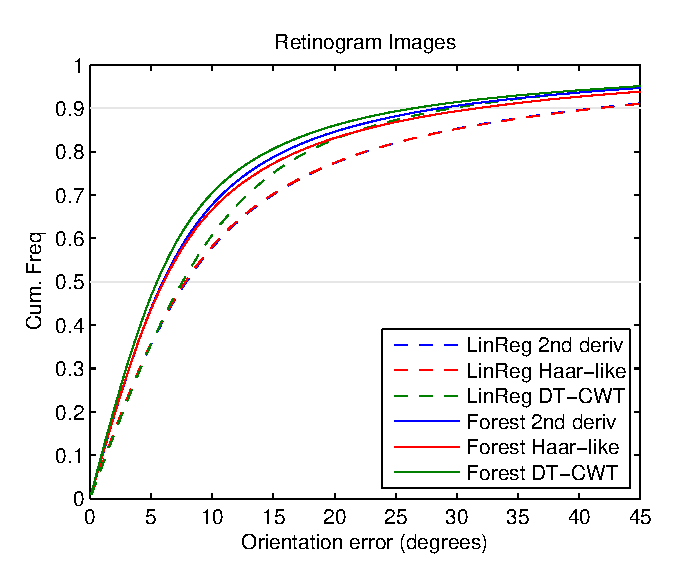
\includegraphics[width=0.48\columnwidth]{\figpath/retina/retinogram_expt} &
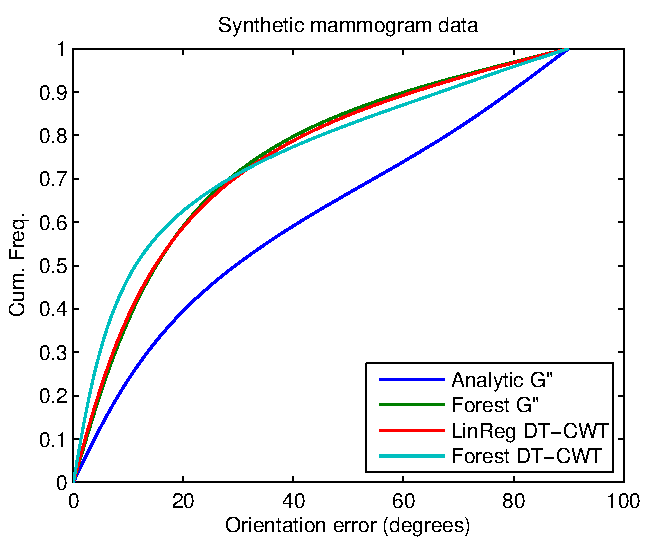
\includegraphics[width=0.48\columnwidth]{\figpath/mammo/mammography_expt} \\
(a) & (b) \\
\end{tabular}
%
\caption{Cumulative frequency of angular error for (a) retinogram images and (b) synthetic mammogram-like images.}
\label{f:cumfreq}
\end{figure}

Comparing performance for the various combinations (\fref{f:cumfreq}a and \tref{t:retinopathy}), we see that in general the analytic methods perform poorly in comparison with the regression approaches, that Random Forests outperform other regression methods and that the \dtcwt~is superior to other feature representations. With the exception of the boosted regressor, the Haar-like approximation exhibited similar performance to the second derivative, suggesting that it may be used effectively in scenarios where efficiency is a concern.

It may be surprising just how poorly the analytic formulations perform in contrast to the regressors. On inspection of the outputs, we see that the monogenic signal (based on first derivatives) does indeed fail at the centre of linear structures. Since, however, many of the vessels in the retinograms are a single pixel in width (such that anywhere on the line is at the centre by definition) the monogenic signal is doomed. The regressors also get some benefit from pooling responses over several pixels.

As noted earlier, when using squared or second derivative responses it is necessary to compute the responses at the two possible solutions to determine which is the correct one. With the Haar-like approximation that combines the response to $\Ixx$ and $\Iyy$, this analytic solution is not available and a regression approach becomes necessary. Also, since the linear regressor minimizes the average error it contains no mechanism for selecting the correct orientation in this way. This is likely to be one reason for its poor performance relative to more sophisticated regressors such as the Random Forest. There is a penalty, however, in efficiency when using complex regressors like the Random Forest.


\subsection{Mammogram-like Images}
\label{s:expts_synth_mammography}
\begin{table}[t]
\centering
\begin{tabular}{l|c c c c}
							& \multicolumn{4}{c}{Feature Type} \\
							& Monogenic		& 2nd deriv.	& Haar				& \dtcwt \\
\hline
\input{mammography_table.txt}
\end{tabular}
%
\caption{Median absolute error (degrees) for combinations of input feature and regressor on 100 synthetic mammogram images.}
\label{t:synth_mammography}
\end{table}

As vessels are often clearly visible in retinograms, we repeated this experiment on a more challenging dataset of synthetic images that realistically approximate the structure of mammographic images. More specifically, we sampled a background by cropping a $512{\times}512$ image region from a real mammogram upon which we superimposed one or more lines of varying orientation, contrast, width and profile (\fref{f:synth_mammography}a). As the lines were synthetic, we had access to both a mask (\fref{f:synth_mammography}b) and ground truth orientation for the superimposed structure.

As in the retinogram experiment, we sampled 200000 pixels from such images and computed a feature vector for each with which we trained a regressor. We then applied every trained regressor for every feature type to a fixed set of 100 synthesized images and computed the error at the known foreground pixel positions (\fref{f:synth_mammography}c). As before, Random Forests and the \dtcwt~outperform other methods, though errors were generally higher on account of the more challenging data (\fref{f:cumfreq}b and \tref{t:synth_mammography}). We also note that although the median error for the Random Forest was lower for the \dtcwt~than the second derivatives, the situation was reversed for higher percentiles (\ie~the graphs cross). We care less, however, about differences between errors above a certain threshold (it matters little whether the estimate is out by $60^\circ$ or $70^\circ$ -- they are both terrible estimates) so it may be argued that the Random Forest performs better over the region in which we are interested.

\begin{figure}[t]
\centering
\begin{tabular}{c c c}
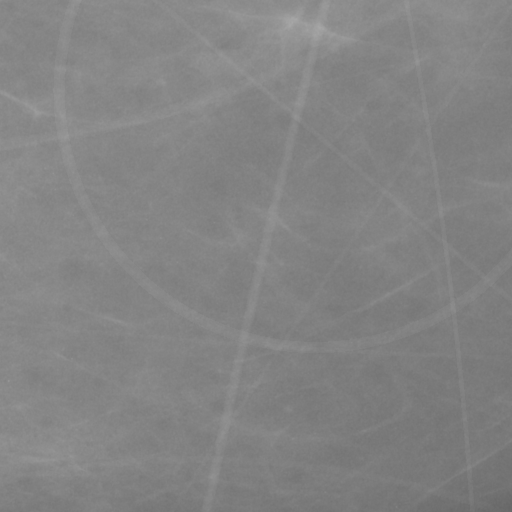
\includegraphics[width=0.3\columnwidth]{\figpath/mammo/synth_lines} &
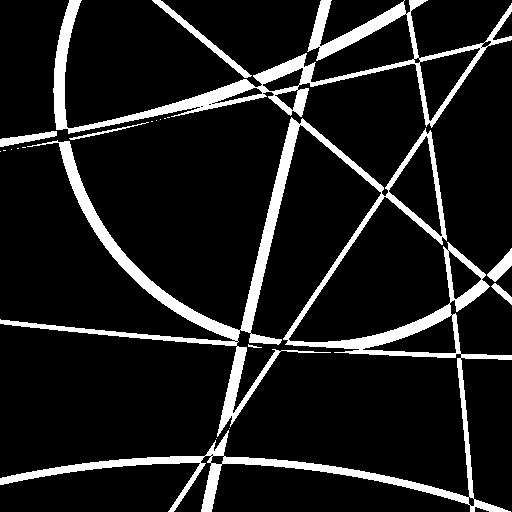
\includegraphics[width=0.3\columnwidth]{\figpath/mammo/synth_mask} &
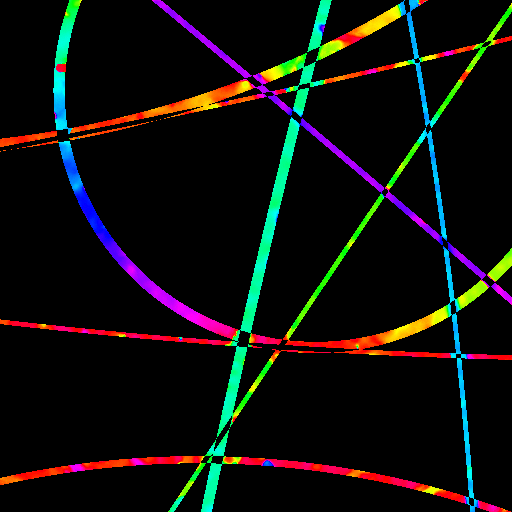
\includegraphics[width=0.3\columnwidth]{\figpath/mammo/synth_result} \\
(a) & (b) & (c)
\end{tabular}
%
\caption{Synthetic mammographic images: %
(a) input image; %
(b) mask indicating pixels belonging to a vessel; %
(c) orientation (indicated by colour) estimated using Random Forest regression over \dtcwt~features. The mask was not used to estimate orientation.%
}
\label{f:synth_mammography}
\end{figure}

\begin{figure}[t]
\centering
\begin{tabular}{c c}
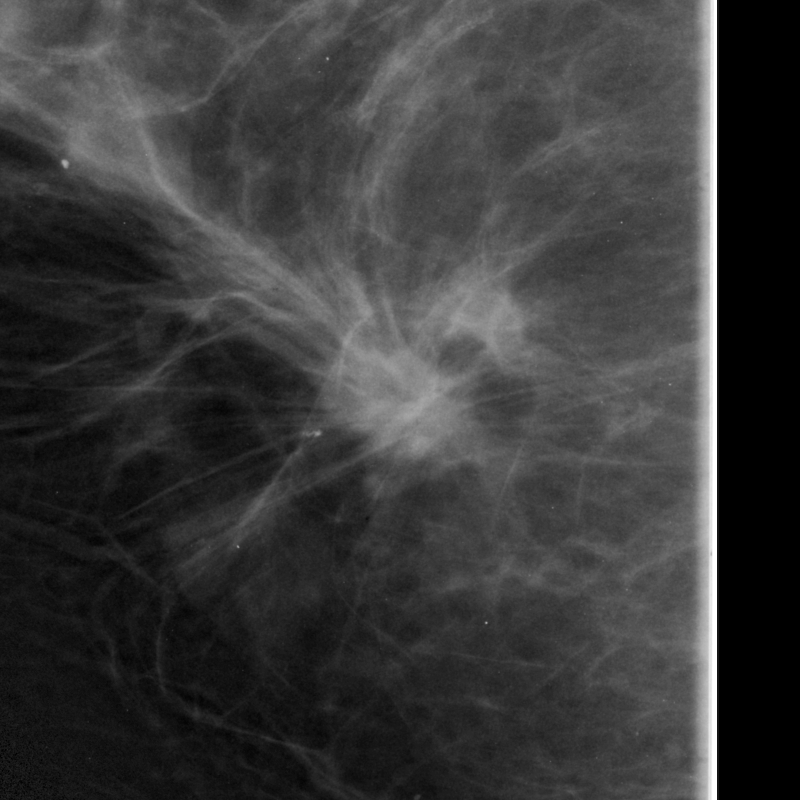
\includegraphics[width=0.3\columnwidth]{\figpath/mammo/024RCC_roi} &
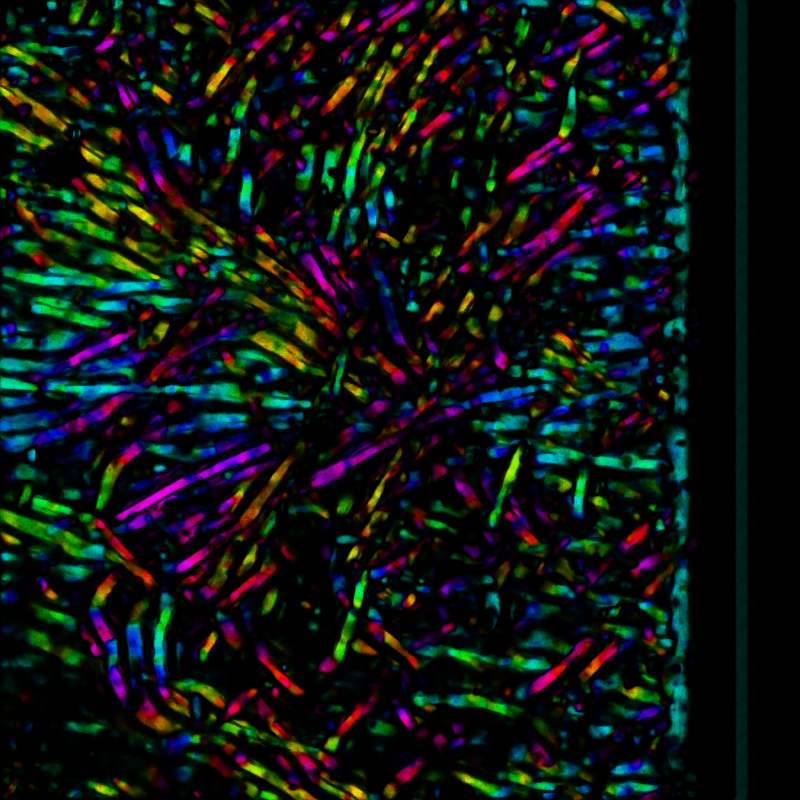
\includegraphics[width=0.3\columnwidth]{\figpath/mammo/024RCC_roi_class_ori_masked} \\
(a) & (b) \\
\end{tabular}
%
\caption{Real mammographic images: %
(a) input image; %
(b) estimated orientation from a Random Forest using \dtcwt~features. Hue indicates the estimated orientation and brightness is determined by the confidence in the estimate (as quantified by the dispersion).}
\label{f:real_mammography}
\end{figure}

% CLAIM: that the separable filters are faster than nonseparable ones (but by how much?)
% CLAIM: that the Haar-like features are faster than separable filtering
In terms of efficiency, we recorded the mean time (using Matlab on a 2.66Ghz, quad-core desktop PC with 3.25Gb RAM) over 20 images for five feature representations: the monogenic signal (2.96\emph{s}); non-separable second derivatives (3.71\emph{s}); separable second derivatives (2.04\emph{s}); their Haar-like approximations (2.35\emph{s}); and the \dtcwt (19.96\emph{s}). Unsurprisingly, under test conditions the separable filters were indeed faster than their non-separable counterparts while the \dtcwt~was an order of magnitude slower than the separable filters. The Haar-like approximations were comparable to but slower than the separable filters, though the separable filters did exploit the built-in (\ie~compiled) convolution functions in Matlab; we expect that an optimized implementation of the Haar-like features would offer similar performance gains as observed in face detection applications~\cite{Viola_Jones_IJCV04}.
%%% This is a pretty weak conclusion to the experiment but the best we can expect at this point. Also, if you need to use a regressor as slow as the RF to get accuracy that is comparable to the analytic second derivatives then the small difference in filtering time becomes irrelevant}

Having trained regressors on synthetic mammogram-like images, we can also apply them to real mammograms. In a region of interest surrounding a spiculated lesion, the linear structures radiating from the central mass are clearly visible when weighted by the confidence in their orientation estimation (\fref{f:real_mammography}).


\subsection{Fingerprint Analysis}
\label{s:expts_fingerprints}
Noting that estimating orientation is of interest to the fingerprint analysis community, we briefly present some results that highlight the difference in performance between using filters based on first and second derivatives, respectively. As discussed earlier, the estimated orientation using gradient based filters~\cite{Bazen_Gerez_TPAMI02,Mei_etal_IVC09} -- the mainstay of fingerprint orientation analysis -- becomes unstable near the centre of a symmetric bar feature (\fref{f:fingerprints}c), whereas a filter based on second derivatives remains stable. There are, however, artefacts around the edges of the ridge features for the second derivative that may suggest a solution based on both types.

\begin{figure}[t]
\centering
\begin{tabular}{c c c}
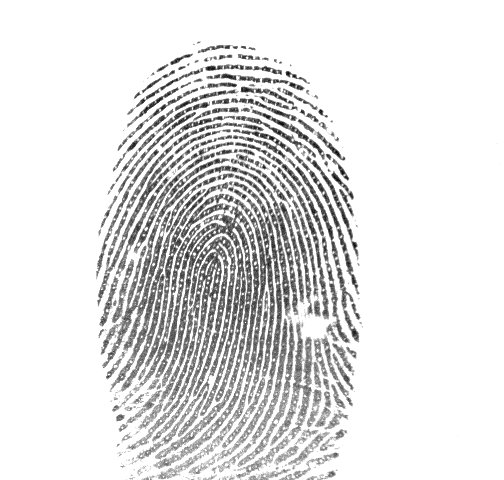
\includegraphics[width=0.3\columnwidth]{\figpath/fingerprint/input} &
%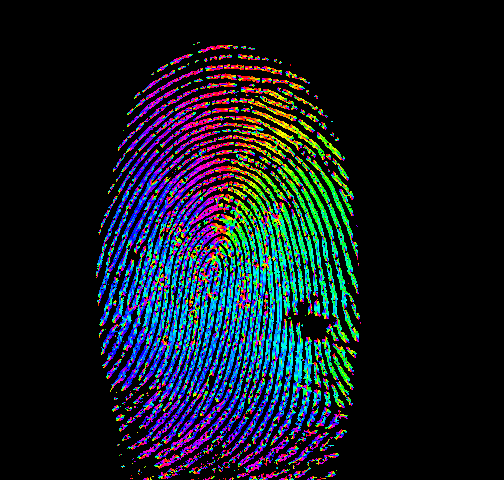
\includegraphics[height=0.15\textheight]{\figpath/fingerprint/ori_1st} &
%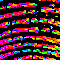
\includegraphics[height=0.15\textheight]{\figpath/fingerprint/ori_1st_zoom} \\
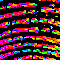
\includegraphics[width=0.3\columnwidth]{\figpath/fingerprint/ori_1st_zoom} &
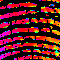
\includegraphics[width=0.3\columnwidth]{\figpath/fingerprint/ori_clover_zoom} \\
(a) & (b) & (c) \\
%&
%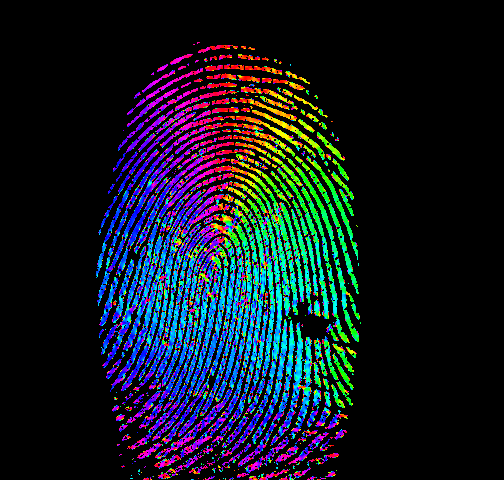
\includegraphics[height=0.15\textheight]{\figpath/fingerprint/ori_clover} &
%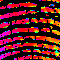
\includegraphics[height=0.15\textheight]{\figpath/fingerprint/ori_clover_zoom} \\
%		& (d) & (e)
\end{tabular}
%
\caption{Fingerprint images: %
(a) input image; %
(b,c) first derivative estimate of orientation with close-up; %
(d-e) second derivative estimate with close-up. Note the high errors at the centre of the ridge for first derivatives and at the edges of the ridge for second derivatives.}
\label{f:fingerprints}
\end{figure}


%\section{Discussion}
%\label{s:discussion}
%
%\begin{figure}[t]
%	\centering
%		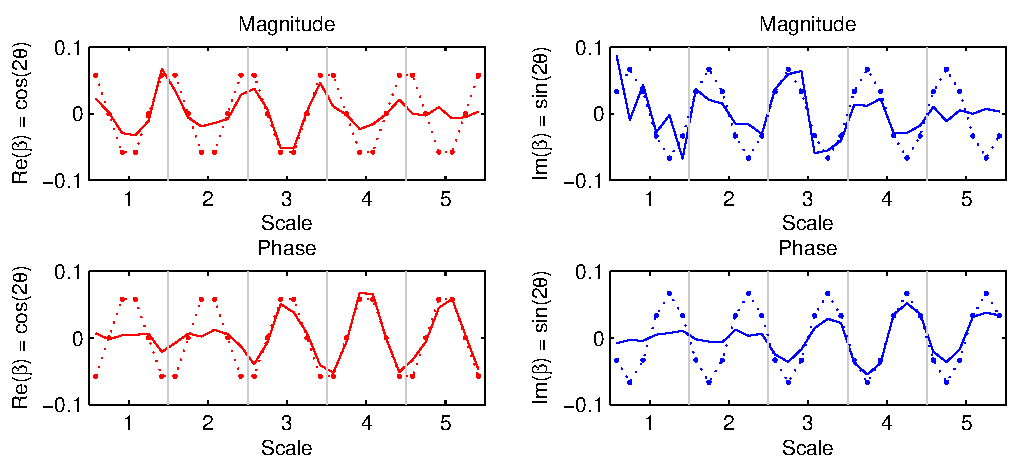
\includegraphics[width=0.9\columnwidth]{\figpath/linreg_coeffs}
%	\caption{Linear regression coefficients for (left) $\cos 2\theta$ and (right) $\sin 2\theta$, using (top) response magnitude and (bottom) response phase.}
%	\label{f:linreg_coeffs}
%\end{figure}



\section{Conclusions}
\label{s:conclusions}
From these experiments, we can make several conclusions. First, we see that filters based on first derivatives do indeed perform poorly near the centre of a ridge feature (\fref{f:fingerprints}b); second derivatives are much better, though they result in artefacts at the edges (where we are less concerned). Second, there is potential to approximate the second derivative filter responses with Haar-like features if efficiency is a key concern, though it is less clear how to combine these responses to give a unique solution. Of the filters we tested, we found that the \dtcwt~gave the best results regardless of the regressor used, though was significantly more computationally expensive. Of the regressors we tested, Random Forests performed best and we have provided some insight as to why alternatives (\eg~linear regression) perform less well. We must, however, take care when building regressors for orientation prediction in order to ensure that angles wrap around the circle correctly.

%\end{document}

\bibliography{./bib/_aliases,./bib/mobio,./bib/mammography,./bib/ml,/bib/local}

\end{document}

\clearpage
\appendix
\section{Derivations}
Defining $\G_{(1)}(\theta)$ as the first derivative filter at angle $\theta$,
%
\begin{align}
\G_{(1)}(\theta)
	&= 	\frac{\partial G}{\partial r} \\
	&= 	\frac{\partial G}{\partial x}\frac{\partial x}{\partial r} +
			\frac{\partial G}{\partial y}\frac{\partial y}{\partial r} \\
	&= 	\Gx \cos(\theta) + \Gy \sin(\theta)
\label{e:dG}
\end{align}

\noindent where $\Gx = \G_{(1)}(0^\circ)$ and $\Gy = \G_{(1)}(90^\circ)$ (\fref{f:filters}). We can write the response to this filter as
%
\begin{align}
R_{(1)}(\theta)
	&= 	\G_{(1)}(\theta) \ast I \\
	&=	(\Gx \cos(\theta) + \Gy \sin(\theta)) \ast I \\
	&=	(\Gx \ast I) \cos(\theta) + (\Gy \ast I) \sin(\theta)) \\
	&=	\Ix \cos(\theta) + \Iy \sin(\theta)
\label{e:R1}
\end{align}

\noindent such that differentiating and equating to zero gives
%
\begin{align}
\frac{d}{d\theta}R_{(1)}
	&= -\Ix \sin(\theta) + \Iy \cos(\theta) = 0 \\
\Rightarrow \tan(\theta)
	&= \frac{\Iy}{\Ix}.
\label{e:t1}
\end{align}



\begin{align}
R_{(1)}^2(\theta)
	&=	(\Ix \cos(\theta) + \Iy \sin(\theta))^2 \\
	&= 	\Ix^2 \cos^2(\theta)+\Iy^2 \sin^2(\theta)+2\Ix\Iy\sin(\theta)\cos(\theta) \\
	&= 	\Ix^2 \cos^2(\theta)+\Iy^2 \sin^2(\theta)+\Ix\Iy\sin(2\theta)
\label{e:R1sqr}
\end{align}

\noindent such that differentiating and equating to zero gives
%
\begin{align}
\frac{d}{d\theta}R_{(1)}^2
	&= 	-2\Ix^2 \cos(\theta)\sin(\theta) + 2\Iy^2 \sin(\theta)\cos(\theta) + 2\Ix\Iy\cos(2\theta) \\
	&= 	(\Iy^2-\Ix^2) \sin(2\theta) + 2\Ix\Iy\cos(2\theta) = 0 \\
\Rightarrow \tan(2\theta)
	&= 	\frac{2\Ix\Iy}{\Ix^2-\Iy^2}.
\label{e:t1sqr}
\end{align}


Squared filters:

\begin{align}
\tan(2\theta)
	&= 	\frac{2(\Gx\Gy \ast I)}{(\Gx^2 \ast I)-(\Gy^2 \ast I)}.
\label{e:t1fsqr}
\end{align}

\noindent with `cloverleaf' type filters.

Second derivs:
%
\begin{align}
\G_{(2)}(\theta)
	&= 	\frac{\partial}{\partial x}(\Gx \cos(\theta) + \Gy \sin(\theta))\frac{\partial x}{\partial r} +
			\frac{\partial}{\partial y}(\Gx \cos(\theta) + \Gy \sin(\theta))\frac{\partial y}{\partial r} \\
	&= 	(\Gxx \cos(\theta) + \Gyx \sin(\theta))\cos(\theta) +
			(\Gxy \cos(\theta) + \Gyy \sin(\theta))\sin(\theta) \\
	&= 	\Gxx\cos^2(\theta) + \Gyy\sin^2(\theta) + 2\Gxy\sin(\theta)\cos(\theta) \\
	&=	\Gxx\cos^2(\theta) + \Gyy\sin^2(\theta) + \Gxy\sin(2\theta) \\
\label{e:ddG}
\end{align}

\noindent where the response to this filter is
%
\begin{align}
R_{(2)}(\theta)
	&= 	\G_{(2)}(\theta) \ast I \\
	&=	\Ixx\cos^2(\theta) + \Iyy\sin^2(\theta) + \Ixy\sin(2\theta)
\label{e:R2}
\end{align}

\noindent with a stationary point at

\begin{align}
\frac{d}{d\theta}R_{(2)}
	&= 	-2\Ixx\cos(\theta)\sin(\theta) + 2\Iyy\sin(\theta)\cos(\theta) + 2\Ixy\cos(2\theta) \\
	&= 	(\Iyy-\Ixx)\sin(2\theta) + 2\Ixy\cos(2\theta) = 0 \\
\Rightarrow \tan(2\theta)
	&= 	\frac{2\Ixy}{\Ixx-\Iyy}.
\label{e:t2}
\end{align}


\end{document}
